\documentclass[ngerman,hyperref={pdfpagelabels=false}]{beamer}

% -----------------------------------------------------------------------------

\graphicspath{{images/}}

% -----------------------------------------------------------------------------

\usetheme{KIT}

\setbeamercovered{transparent}
%\setbeamertemplate{enumerate items}[ball]

\newenvironment<>{KITtestblock}[2][]
{\begin{KITcolblock}<#1>{#2}{KITblack15}{KITblack50}}
{\end{KITcolblock}}

\usepackage[ngerman,english]{babel}
\usepackage[utf8]{inputenc}
\usepackage[TS1,T1]{fontenc}
\usepackage{array}
\usepackage{multicol}
\usepackage[absolute,overlay]{textpos}
\usepackage{beamerKITdefs}

\pdfpageattr {/Group << /S /Transparency /I true /CS /DeviceRGB>>}	%required to prevent color shifting withd transparent images


\title{Algorithmen I - Tutorium 13/13}
\subtitle{Sebastian Schmidt -- \textit{isibboi@gmail.com}}

\author[Sebastian Schmidt]{Sebastian Schmidt}
\institute{Arbeitsgruppe Kryptographie und Sicherheit}

\TitleImage[width=\titleimagewd,height=\titleimageht]{titel}

\KITinstitute{Arbeitsgruppe Kryptographie und Sicherheit}
\KITfaculty{Fakult\"at f\"ur Informatik}

% -----------------------------------------------------------------------------

\begin{document}
\setlength\textheight{7cm} %required for correct vertical alignment, if [t] is not used as documentclass parameter


% title frame
\begin{frame}
  \maketitle
\end{frame}


\begin{frame}{Dynamische Programmierung}
\begin{itemize}
\item Zur Lösung von Optimierungsproblemen
\item Optimale Lösung setzt sich aus optimalen Lösungen von Teilproblemen zusammen
\end{itemize}

\begin{enumerate}
\item Direktes Lösen kleinster Teilprobleme
\item Löse nächstgrößere Teilprobleme, bis Lösung für das Ursprüngliche Problem gefunden
\end{enumerate}
\end{frame}

\begin{frame}{Algorithmus von Floyd}
$w[i, j]$ ist die Gewichtsmatrix des Graphen.

$d[i, j]$ ist der aktuelle kürzeste Weg von $i$ nach $j$, der nur über Knoten $<k$ führt.

\vspace{1em}

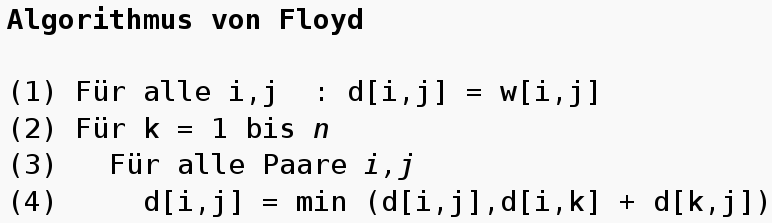
\includegraphics[width=\textwidth]{floyd}
\end{frame}

\begin{frame}{Branch-and-Bound}
Branch and Bound für TSP. Tafel.
\end{frame}

\begin{frame}{Wiederholung}
Fragen? :)
\end{frame}

\begin{frame}
\vspace{-4em}
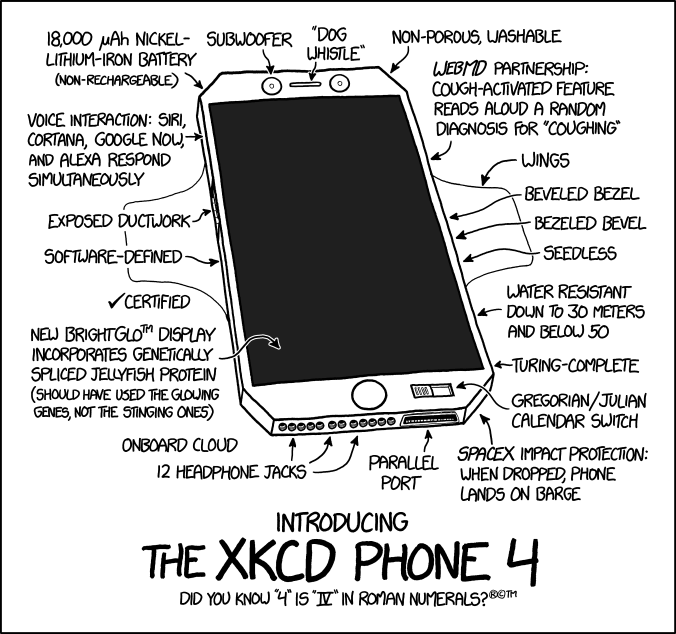
\includegraphics[width=0.87\textwidth]{xkcd_phone_4}
\end{frame}

\end{document}
